% DRAFT v0.1 (2026-09-25). Every number comes from paper/analysis.py -> stats.json / tables.tex,
% or from experiments/02_quantization/ (see AUDIT_LOG.md). Do not edit numbers by hand: re-run analysis.py.
% Build: upload this folder to Overleaf with the official ACL style files (acl.sty, acl_natbib.bst)
% from https://github.com/acl-org/acl-style-files, or place them next to this file.
\documentclass[11pt]{article}
% Use [review] for anonymous conference submission, [final] for arXiv/sharing.
\usepackage[final]{acl}
\usepackage{times}
\usepackage{latexsym}
\usepackage[T1]{fontenc}
\usepackage[utf8]{inputenc}
\usepackage{microtype}
\usepackage{booktabs}
\usepackage{graphicx}
\usepackage{amsmath}

% Title changed from "The Tokenizer Tax Compounds..." to avoid confusion with Srivastava (2026),
% "The Tokenizer Tax" (arXiv 2607.24276). Working title, open to revision.
\title{Taxed Twice: Tokenizer Parity Predicts 4-bit Quantization Damage\\in Indic Language Models}

\author{Shrey Sati \\
  JSS University, Noida, India \\
  \texttt{shrey.sati@gmail.com}}

\begin{document}
\maketitle

\begin{abstract}
Running language models locally, on laptops, phones and edge devices, typically means running small, quantized ones. We ask whether 4-bit quantization degrades Indian languages uniformly. Across 7 open models of 1--3B parameters (four global, three Indic-built) and 11 languages (English and 10 Indic languages), on 256 parallel sentences from IN22-Gen, we find that a language's \emph{tokenizer tax}, its token count relative to the same content in English, strongly predicts how much its per-character negative log-likelihood degrades under NF4 quantization (Spearman $\rho=0.71$, $p<10^{-4}$ by a within-model permutation test). The relationship holds after removing each model's overall fragility ($\rho=0.65$). In Pragna-1B, languages absent from training but tokenized efficiently degrade about as little as a trained language, while poorly tokenized untrained languages degrade four times more. Translation experiments confirm that 4-bit quantization reliably lowers output quality (43 of 50 model--language--direction cells show a significant drop), but at 1--3B scale the size of the drop is only loosely predicted by likelihood damage, partly because of floor effects. We release all code, per-sentence results, and a reproducibility log.
\end{abstract}

\section{Introduction}
Running a language model locally, on consumer GPUs, laptops or edge devices, typically means running a small, quantized one: 8- and 4-bit quantization is what lets 1--4B models fit such hardware~\citep{dettmers2022int8,dettmers2023qlora}. Local deployment matters wherever data cannot leave an organisation or connectivity is limited. Yet quantization is usually evaluated in English. \citet{marchisio2024quantization} showed that quantization affects languages unequally, with non-Latin scripts hit hardest, in models where script and training-data share move together.

Separately, tokenizers are known to charge some languages far more tokens for the same content, which raises cost and latency and shrinks usable context~\citep{petrov2023tokenizers,ahia2023cost,rust2021tokenizer}. For Indian languages this \emph{tokenizer tax} has been quantified directly: \citet{srivastava2026tokenizertax} reports an average 8.0$\times$ overhead relative to English under cl100k\_base on FLORES-200, and \citet{brahma2025indictok} study how tokenizer design choices affect 17 Indic languages. Tokenization also shapes model behaviour beyond cost: \citet{ghosh2026noncanonical} show that the invariance to alternative tokenizations observed for English does not generalize across 27 languages, and \citet{uppadhyay2026depart} attribute most language-level variance in multilingual LLM performance to observable features such as script and language family. These works measure the tax and its effects at full precision. We ask what it costs \emph{after} compression. Indic languages are among the most heavily taxed by global tokenizers, and Indic-built models such as Sarvam-1 and BharatGen's PARAM-1 explicitly target tokenizer efficiency for Indian languages~\citep{sarvam2024sarvam1,pundalik2025param1}.

We connect the two: \textbf{does the tokenizer tax also predict how much a language breaks under quantization?} Our contributions:
\begin{enumerate}
\item A controlled study of 7 open 1--3B models $\times$ 11 languages at bf16, int8 and NF4, on parallel sentences, with sentence-level bootstrap confidence intervals.
\item Evidence that tokenizer parity predicts NF4 likelihood damage across and within models, including a disentangling case (Pragna-1B) where tokenization and training coverage come apart.
\item A translation study in both directions showing that the damage is real in generation but only loosely predicted at this scale, and an honest account of why.
\end{enumerate}

\section{Setup}
\paragraph{Models.} Global: Llama-3.2-1B and -3B~\citep{grattafiori2024llama3}, Gemma-3-1B~\citep{gemma2025gemma3}, Qwen3-1.7B-Base~\citep{yang2025qwen3}. Indic-built: Sarvam-1 (2.5B; 10 Indic languages + English)~\citep{sarvam2024sarvam1}, Pragna-1B (Hindi, Bangla, Gujarati, English)~\citep{soket2024pragna}, and PARAM-1-2.9B (Hindi + English)~\citep{pundalik2025param1}. We use base checkpoints except PARAM-1, for which only the instruct checkpoint is public. Exact model revisions are listed in the appendix.

\paragraph{Data.} The first 256 sentences of IN22-Gen~\citep{gala2023indictrans2} (CC-BY-4.0), which provides the same content in English and all 22 scheduled Indian languages. We use English, Hindi, Bengali, Marathi, Gujarati, Punjabi, Odia, Tamil, Telugu, Kannada and Malayalam.

\paragraph{Quantization.} bitsandbytes LLM.int8() (default outlier threshold 6.0)~\citep{dettmers2022int8} and 4-bit NF4 with bf16 compute~\citep{dettmers2023qlora}, compared against a bf16 baseline. PARAM-1 was run only at bf16 and NF4 (Section~\ref{sec:limits}).

\paragraph{Damage metric.} For each sentence we sum the token-level negative log-likelihood (nats) under teacher forcing and divide the total over sentences by the total character count (NLL/char). This normalises by content rather than by tokens, so languages and tokenizers are comparable within a language. Damage is the absolute change $\Delta = \text{NLL/char}_{q} - \text{NLL/char}_{\text{bf16}}$. We report absolute rather than relative change because relative change inflates languages with a low baseline. Sentences are never truncated.

\paragraph{Tokenizer tax.} Parity is the token count of a language divided by that of English over the same 256 sentences, for each model's own tokenizer.

\paragraph{Statistics.} 95\% confidence intervals come from 2,000 paired bootstrap resamples over sentences. Pooled correlations are Spearman's $\rho$. Their significance is tested by permuting parity \emph{within} each model (10,000 permutations), which preserves each model's overall level of damage.

\section{Results}
\begin{figure}[t]
  \centering
  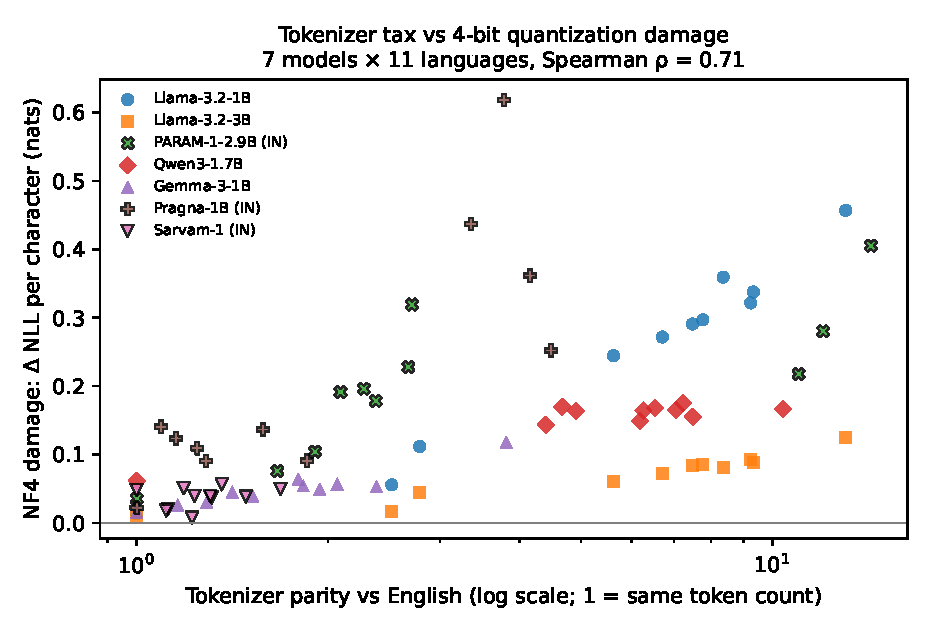
\includegraphics[width=\columnwidth]{figures/fig1_parity_vs_damage.pdf}
  \caption{Tokenizer parity (log scale) against NF4 damage in NLL per character, for 7 models $\times$ 11 languages. Indic-built models are outlined.}
  \label{fig:main}
\end{figure}

\begin{table}[t]
  \centering\small
  \resizebox{\columnwidth}{!}{\begin{tabular}{lrrrrr}
\toprule
Model & Parity & Eng.\ $\Delta$ & Indic mean $\Delta$ & Indic max $\Delta$ & $\rho$ \\
\midrule
Sarvam-1$^\dagger$ & 1.3 & 0.048 & 0.036 & 0.056 & 0.32 \\
Gemma-3-1B & 1.9 & 0.016 & 0.054 & 0.118 & 0.85 \\
Pragna-1B$^\dagger$ & 2.4 & 0.022 & 0.236 & 0.618 & 0.67 \\
Param-1-2.9B$^\dagger$ & 5.3 & 0.035 & 0.220 & 0.405 & 0.93 \\
Qwen3-1.7B & 6.5 & 0.061 & 0.162 & 0.175 & 0.51 \\
Llama-3.2-3B & 7.3 & 0.008 & 0.075 & 0.125 & 0.96 \\
Llama-3.2-1B & 7.3 & 0.014 & 0.275 & 0.457 & 0.97 \\
\bottomrule
\end{tabular}}
  \caption{Per-model NF4 damage ($\Delta$ NLL/char, nats). Parity = mean Indic parity. $\rho$ = within-model Spearman between parity and damage over 11 languages. $^\dagger$Indic-built.}
  \label{tab:models}
\end{table}

\paragraph{Int8 is nearly free; NF4 is not.} Across the six models run at both precisions, mean int8 damage is 5--14$\times$ smaller than NF4 damage. We therefore focus on NF4.

\paragraph{The tokenizer tax predicts NF4 damage.} Pooled over 77 model--language points, parity and NF4 damage correlate at $\rho=0.71$ ($p<10^{-4}$; Figure~\ref{fig:main}). With one intercept per model, damage increases by 0.077 nats/char (95\% CI 0.058--0.101) per doubling of parity (0.11 per unit of natural-log parity). To separate language effects from model fragility, we subtract each model's English damage from its Indic damage: the correlation remains $\rho=0.65$ ($p<10^{-4}$). Within models, the relationship is strongest where parity varies most (Llama-3.2-1B $\rho=0.97$, Llama-3.2-3B 0.96, PARAM-1 0.93) and weakest for Sarvam-1 (0.32), whose tokenizer is nearly flat across languages (Table~\ref{tab:models}).

\paragraph{Same size, different tokenizer.} Llama-3.2-1B and Gemma-3-1B lose similar amounts in English (0.014 vs 0.016), but Tamil loses 0.297 under Llama and 0.039 under Gemma, whose tokenizer is far more economical for Indic scripts. Scale shrinks the effect without removing it: from Llama-3.2-1B to -3B, mean Indic damage falls from 0.275 to 0.075 but the ranking of languages is preserved ($\rho=0.96$).

\paragraph{Disentangling tokenization from training data.} Tokenizer parity and training-data share are correlated, since poorly tokenized languages are usually also under-represented in training. Pragna-1B lets us separate them, because it was trained only on Hindi, Bangla, Gujarati and English. Among its \emph{untrained} languages, those it tokenizes efficiently (Tamil, Marathi, Kannada; parity $<2$) lose 0.10 on average, about the same as trained Hindi (0.11), while poorly tokenized untrained languages (Punjabi, Odia, Telugu, Malayalam; parity 3.4--4.5) lose 0.42. This is a single model and should be read as suggestive, but it points to tokenization as a factor beyond training coverage.

\paragraph{Indic-built tokenizers largely avoid the effect.} Sarvam-1, with the lowest parity (mean 1.3), shows small NF4 damage in every Indic language ($\le$0.056; Tamil 0.008). PARAM-1 illustrates the flip side: it is efficient for Hindi (parity 1.7, damage 0.076) but not for scripts outside its training (Gujarati, Punjabi and Odia at parity 11--14), which are among its most damaged languages.

\section{Does the damage show up in generation?}
We translate 128 sentences Indic$\to$English and 64 sentences English$\to$Indic (3-shot, greedy; shots are IN22-Gen rows 1000--1002, disjoint from the test rows) in five languages (Hindi, Bengali, Tamil, Telugu, Odia) with five models: Llama-3.2-1B, Gemma-3-1B, Qwen3-1.7B, Sarvam-1 and Pragna-1B. Llama-3.2-3B exceeded our 8\,GB GPU at bf16 during generation, and PARAM-1 was not included in this experiment (it runs only in a separate environment with an older library version, and its only public checkpoint is instruction-tuned). Outputs are scored with chrF++~\citep{popovic2017chrfpp} via SacreBLEU~\citep{post2018sacrebleu} (signature in Appendix~\ref{app:repro}). NF4 lowers quality in both directions: the drop's 95\% CI excludes zero in 22/25 cells (Indic$\to$English) and 21/25 cells (English$\to$Indic), with mean drops of 3.4 and 3.5 chrF++.

The \emph{size} of the drop, however, is only loosely predicted. For Indic$\to$English, per-model drops track each model's damage to \emph{English} (the output language) more than its Indic likelihood damage. For English$\to$Indic, many cells sit near the floor: 14 of 25 have bf16 chrF++ below 20, where a model already produces poor output and cannot degrade much further. Among the 11 non-floor cells, the drop correlates with parity ($\rho=0.67$) and likelihood damage ($\rho=0.57$), but this sample is too small to rely on. Sarvam-1 is a notable case: its likelihood damage is small, yet its chrF++ drops by about 4 points in both directions. Teacher-forced likelihood appears to understate generation damage there, consistent with \citet{marchisio2024quantization}'s finding that automatic metrics underestimate the harm of quantization.

\section{Discussion and recommendations}
Tokenizer inefficiency is usually framed as a cost: more tokens, higher latency, less context. Our results suggest a second, compounding cost: token-hungry languages also lose more when the model is compressed. In practice: (i) if a deployment serves Indic languages, prefer int8 over NF4 for small models, or (ii) use a model whose tokenizer is efficient for the target language; (iii) evaluate quantized models in the deployment language, not only in English; and (iv) do not rely on likelihood alone, because generation can degrade more than likelihood suggests.

\section{Limitations}
\label{sec:limits}
(1) Our main metric is teacher-forced likelihood, and generation results only partially follow it. (2) NLL per character is not comparable across scripts, so we compare only changes within a language. (3) Parity and training-data share are confounded. The Pragna analysis separates them in one model only. (4) We test one quantization family (bitsandbytes int8/NF4), not GGUF, GPTQ or AWQ. (5) All models are 1--3B, and the effect shrinks with scale (1B$\to$3B), so larger models may behave differently. (6) PARAM-1 is an instruct checkpoint, was run with an older library version for compatibility, and has no int8 or translation run. (7) One dataset (general-domain IN22-Gen), first 256 sentences. (8) Confidence intervals reflect sentence sampling only. (9) Translation covers five models, and many English$\to$Indic cells are near the floor. Testing 7B+ models, where Indic generation clears this floor, is the natural next step and is beyond an 8\,GB laptop GPU.

\section*{Reproducibility and AI assistance}
All experiments ran on one laptop (RTX 5060, 8\,GB). Code, per-sentence outputs, exact library versions, model revisions and an audit log of every run, change and corrected error are released at \url{https://github.com/satanrayshe/taxed-twice}. The author designed the study and made its decisions with substantial help from an AI assistant (Claude, Anthropic) for code, analysis and drafting. All results were checked by the author, and all citations were verified against their sources.

\bibliography{refs}

\appendix
\section{Reproducibility details}
\label{app:repro}
\paragraph{chrF++ signature (SacreBLEU).} \texttt{nrefs:1\allowbreak|case:mixed\allowbreak|eff:yes\allowbreak|nc:6\allowbreak|nw:2\allowbreak|space:no\allowbreak|version:2.6.0}

\paragraph{Model revisions.}
Hugging Face commit hashes (2026-09-24): Sarvam-1 e9607337; Llama-3.2-1B 4e20de36; Llama-3.2-3B 13afe512; Gemma-3-1B-pt fcf18a2a; Qwen3-1.7B-Base ea980cb0; Pragna-1B d7375b4c; PARAM-1-2.9B-Instruct f9b32a72; IN22-Gen dataset e042ab3d.

\end{document}
